\documentclass[11pt,letterpaper]{article}
\usepackage[margin=1.2in]{geometry}
\usepackage{amsmath, amssymb}
\usepackage{times}
\usepackage[mathscr]{euscript}
%\usepackage{mathrsfs}
\usepackage{graphicx}
\usepackage{color}
\usepackage[normalem]{ulem}
\usepackage{bm}
\usepackage{epstopdf}
\numberwithin{equation}{section}
\usepackage{mathrsfs}
\usepackage[round]{natbib}
\usepackage{subcaption}
\graphicspath{ {images/} }
 \usepackage[table]{xcolor}
\usepackage{longtable}
\usepackage[margin=1.2in]{geometry}
\usepackage{amsmath, amssymb}
\usepackage{amsthm}
\usepackage{times}
\usepackage[mathscr]{euscript}
%\usepackage{mathrsfs}
\usepackage{graphicx}
\usepackage{color}
\usepackage[normalem]{ulem}
\usepackage{bm}
\usepackage{epstopdf}
\numberwithin{equation}{section}
\usepackage{mathrsfs}
\usepackage[round]{natbib}
\usepackage{subcaption}
\graphicspath{ {images/} }
 \usepackage[table]{xcolor}
\usepackage{longtable}
\usepackage{array}
\usepackage{relsize}
\usepackage{pdflscape}
\usepackage[margin=1.2in]{geometry}
\usepackage{amsmath, amssymb}
\usepackage{times}
\usepackage[mathscr]{euscript}
%\usepackage{mathrsfs}
\usepackage{graphicx}
\usepackage{color}
\usepackage[normalem]{ulem}
\usepackage{bm}
\usepackage{epstopdf}
\numberwithin{equation}{section}
\usepackage{mathrsfs}
\usepackage[round]{natbib}
\usepackage{subcaption}
\graphicspath{ {images/} }
 \usepackage[table]{xcolor}
\usepackage{longtable}
\usepackage{array}
\newcolumntype{P}[1]{>{\centering\arraybackslash}p{#1}}
\usepackage{changepage}
\usepackage[affil-it]{authblk}
\usepackage{multirow, booktabs}
\usepackage{multicol}
\usepackage[nodisplayskipstretch]{setspace}
\usepackage{rotating}

\usepackage{bbm}

\newtheorem{theorem}{Theorem}[section]
\newtheorem{lemma}[theorem]{Lemma}

\begin{document}
\title{\bf Modeling  Frequency and Severity of Claims with the Generalized  Cluster-Weighted Model}

\author{Nikola Po\v cu\v ca, Tatjana Miljkovic,  Petar Jevti\' c, Paul McNicholas  }%Nik: need to add names here.

\maketitle
\doublespacing
\small

\begin{abstract}

In this paper, we propose a generalized cluster-weighted model (GCWM) that allows for modeling non-Gaussian distribution of the continuous covariates and a new zero-inflated GCWM (ZI-GCWM) for modeling insurance claims data with excess zeros. We describe two expectation-optimization (EM) algorithms for parameter estimation in GCWM and ZI-GCWM. A simulation study showed that both cluster models perform well for different settings in contrast to the existing mixture-based approaches. A real data set based on French automobile policies is used to illustrate the application of the proposed models.

\end{abstract}
\textsc{Key Words:} GCWM, CWM, ZI-GCWM, clustering, automobile claims.\\
\textsc{JEL Classification:}  C02, C40, C60.\\
% C02-Mathematical Methods, C40-General mathematical and statistical methods: special topics, c60-General mathematical methods, programming models, mathematical and simulation modeling%
\section{Introduction}\label{sec:introduction}
A significant number of clustering methods have been proposed for sub-grouping the data in the area of computer science, biology, social science, statistics, marketing, etc. \cite{Ingrassia+Punzo+Vittadini+Minotti:2015} proposed a cluster-weighted models (CWMs) as a flexible family of mixture models for fitting the joint distribution of a random vector composed of a response variable and a set of mixed-type covariates with the assumption that continues covariates come from Gaussian distribution. The CWM models with Gaussian assumptions have been proposed by \cite{Gershenfeld:1997}, \cite{Gershenfeld:Schoner+Metois:1999}, and \cite{Gershenfeld:1999} in a context of media technology. Some extensions of this class of models have been considered by \cite{Punzo+Ingrassia:2015}, \cite{Ingrassia+Minotti+Punzo:2014}, and \cite{Ingrassia+Minotti+Vittadini:2012}. These clustering methods luck some capabilities in order to be able to accommodate modeling insurance data (e.g. high excess zeros for claim count, heavy-tail loss distribution, deductible, or limits).

Sub-grouping of insurance policies based on risk classification is a standard practice in insurance. The heterogenous nature of insurance data allows for explorations of many different techniques for sub-grouping risk. As a result, there is a growing number of papers in the area of mixture modeling of univariate and multivariate insurance data to account for heterogeneity of risk. \cite{Lee+Lin:2010}, \cite{Verbelen+Gong+Antonio+Badescu+Lin:2015}, and \cite{Miljkovic+Grun:2016} proposed mixture models for univariate loss data. The idea of mixture modeling of univariate insurance data has been extended to a multivariate classification. A finite mixture of bivariate Poisson regression models with an application to insurance ratemaking was studied by \cite{Bermudez+Karlis:2012}. A Poisson mixture model for count data was considered by \cite{Brown+Buckley:2015} with application in managing Group Life insurance portfolio. \cite{risks_miljkovic} reviewed two complementary mixture-based clustering approaches (cluster-weighted model and mixture-based clustering for an ordered stereotype model) for modeling unobserved heterogeneity in an automobile insurance portfolio, depending on the data structure under consideration. Mixture models with the applications is financial mathematics have been explored by \cite{durham2007sv}, \cite{miljkovic2018new}, and many others.

In this paper paper, we extend the CWM family proposed by \cite{Ingrassia+Punzo+Vittadini+Minotti:2015} to allow for modeling of non-Gaussian continues covariates and a zero-inflated Poisson (ZIP) claims data with excess zeros which are commonly seen in the insurance applications. We define our proposed model as the generalized cluster-weighted model as GCWM and a new zero-inflated GCWM as ZI-GCWM. Two partitioning methods are considered with two separate EM algorithms. The first EM algorithm is for generating the GCWM models, while the second EM is for optimizing the ZI-GCWM. We show that the Bernoulli and Poisson GCWM accurately estimate the initialization of the EM algorithm for the ZI-GCWM model. These models utilize individual policy and claims data and should be useful in the areas of ratemaking and risk management.

This paper is organized as follows. Section 2 presents the proposed model for mixture of GLMs. Section~3 applies the proposed model on a real data of French automobile claims. An extensive simulation study is discussed in Section 4. Conclusion is provided in Section 5.


\section{Proposed Model}

\subsection{Background}

Let $(\bm{X^{'}}, Y)^{'}$  be the pair of a vector of covariates  $\bm{X}$ and a response variable $Y$. Assume this set is defined on some space $\Omega$ that takes values in appropriate Euclidian subspace. Now, assume that there exists $G$ partitions of $\Omega$, denoted as $\Omega_1, \ldots, \Omega_G$.  \cite{Gershenfeld:1997} characterized the cluster-weighted models as a finite mixture of GLMs hence, the joint distribution $f(\bm x, y)$ of $(\bm{X^{'}}, Y )^{'}$  is expressed as follows
 \begin{align}
 f(\bm x, y)= \sum_{j=1}^{G} \tau_j q(y|\bm{x};\Omega_j)p(\bm{x};\Omega_j).
\label{eq1}
\end{align}

The pair $q(y|\bm{x};\Omega_j)$ and $p(\bm{x};\Omega_j)$ are conditional and marginal distributions of $(\bm{X^{'}}, Y)^{'}$ respectively, while $\tau_j$ represents the weight of the $j$th component such that $\sum_{j=1}^{G}\tau_j=1$, $\tau_j>0$.
\cite{Ingrassia+Punzo+Vittadini+Minotti:2015} proposed a flexible family of mixture models for fitting the joint distribution of a random vector $(\bm{X^{'}}, Y)^{'}$ by splitting the covariates into continues and discrete as $ \bm{X}=(\bm{V^{'}},  \bm{W^{'}})^{'}$. This assumption of independence between continues and discrete covariates allows us to multiply their corresponding marginal distributions. Thus, for this setting the model in \eqref{eq1} is reformulated as follows
\begin{align}
 f(\bm x, y; \bm{\Phi})= \sum_{j=1}^{G} \tau_j q(y|\bm{x};\bm{\vartheta_j})p(\bm{x};\bm{\theta_j})=\sum_{j=1}^{G} \tau_j q(y|\bm{x};\bm{\vartheta_j})p(\bm{v}; \bm{\theta_j^{\star}})p(\bm{w};\bm{\theta_j^{\star\star}})
\label{eq2}
\end{align}
where $\bm{v}$ and $\bm{w}$ are the vectors of continues and discrete covariates respectively, the $q(y|\bm{x};\bm{\vartheta_j})$ is a conditional density of $Y|\bm{x}$, with parameter vector $\bm{\vartheta_j}$, the $p(\bm{v};\bm{\theta_j^{\star}})$ is the marginal distribution of $\bm{v}$ with parameter vector $\bm{\theta_j^{\star}}$. the $p(\bm{w};\bm{\theta_j^{\star\star}})$ is the marginal distribution of $\bm{w}$ with parameter vector $\bm{\theta_j^{\star\star}}$. Finally, $\bm{\Phi}:=(\bm{\theta^{\star}},\bm{\theta^{\star\star}}, \bm{\tau}, \bm{\vartheta})$ includes all model parameters. %Nik: this does not seem to be all model parameters? Also, vartheta is either bold face (vector) or not (scalar), and what is $\lm$?. % Notation Corrected - Nik
In addition, the conditional distribution $q(y|\bm{x};\bm{\vartheta_j})$ is assumed to belong to an exponential family of distributions and as such can be modeled in the framework of GLMs. Here, the marginal distribution of continues covariates is assumed to be of Gaussian type. Unfortunately, this last assumption is too strong for use in insurance related applications specifically in rate-making. To relax it, we develop the Generalized cluster-weighted mdoel (GCWM) that allows for non-Gaussian covariates as discussed in the next section.

\subsection{Generalized cluster-weighted model (GCWM) }
We proceed to extend \eqref{eq2} by splitting the  continues covariates further as $\bm{V}:=(\bm U^{'}, \bm T^{'})^{'}$, where $\bm{U}$ is a set of non-Gaussian covariates, and $\bm{T}$ a set of Gaussian  covariates.  Thus (\ref{eq2}) is now recovered as
\begin{align}
 f(\bm x, y; \bm{\Phi})= \sum_{j=1}^{G} \tau_j q(y|\bm{x};\bm{\vartheta_j})p(\bm{t};\bm{\theta_j^{\star}})p(\bm{w};\bm{\theta_j^{\star\star}})p(\bm{u};\bm{\theta_j^{\star\star\star}})
\label{eq3}
\end{align}
which we refer to as generalized cluster-weighted model (GCWM). Here $p(\bm{t};\bm{\theta_j^{\star}})$ denotes the marginal density of Gaussian covariates, with parameter vector $\bm{\theta^{\star}}$, and $p(\bm{u};\bm{\theta_j^{\star\star\star}})$ as the marginal density of the non-Gaussian covariates with parameter vector $ \bm{ \theta_j^{\star\star\star}} $.


As it is relevant to the actuarial application in this paper, we focus on the multivariate log-normal distribution  for non-Gaussian covariates. This however does not reduce the generality of our approach. With log-normal assumption for $p(\bm{u};\bm{\theta_j^{\star\star\star}})$ we have that $\bm{u}$ is defined on $\mathbb{R}_+$ with parameter vector $ \bm{\theta_j^{\star\star\star}} $ having probability density function as
\begin{align} p \left(  \bm{u}; \bm{\theta_j^{\star\star\star}} := ( \bm{\mu_j^{\star\star\star}} ,\bm{ \Sigma _j^{\star\star\star }} ) \right) = \frac{1}{(\prod_{i=1}^{N}u_{i})|\bm{ \Sigma_j^{\star\star\star}} |(2 \pi)^{\frac{p}{2}}}   \exp\left[-\frac{1}{2}(\ln\bm{ u}-\bm{\mu_j}^{\star\star\star})^{'}\bm{\Sigma_j^{{\star\star\star}_{-1}}}(\ln \bm {u}-\bm{\mu_j}^{\star\star\star})\right].
\end{align} The derivation of the equation above can be found in the Appendix \ref{changeVarUni}.

%Nik: is this a density? What range of values of x? What values can mu and sigma take?
% PM: Is this more clear?

\subsection{Zero-inflated Poisson}%Nik: not sure what this means? Specifically, what is the role of the first "-"

In the zero-inflated Poisson model (ZIP) (see \cite{Lambert}) we can split the conditional density $p(y|\bm{x},\bm{\vartheta_j})$ of the response variable $y$, into zero and non-zero densities. %Nik: I don't think "groups" is what is meant.  % Values I meant.
When $y = 0$ the response variable $y$ is distributed with density $q(y = 0|\bm{x},\bm{\vartheta_{j}})$. When $y > 0$ the response variable $y$ is distributed with density $q(y > 0|\bm{x}, \bm{\vartheta_{j}} )$. Given the conditional density now defined for the ZIP model \eqref{eq3}
can be re-written as follows
 \begin{align}
 f(\bm x, y; \Phi)= \sum_{j=1}^{G} \tau_j \left[ q(y = 0|\bm{x};\bm{\vartheta_{j} }) +  q(y > 0|\bm{x} ; \bm{\vartheta_{j}}  ) \right]   p(\bm{t};\bm{\theta_j^{\star}})p(\bm{w};\bm{\theta_j^{\star\star}})p(\bm{u};\bm{\theta_j^{\star\star\star}}).
\end{align}

\newcommand{\xTilda}{\bm{\tilde{x}}}
Let $ \xTilda := [\bm{1},\bm{x}]$, where $\xTilda $ is a matrix of covariates with the addition of a placeholder for the intercept in the GLM. We denote the Poisson conditional density  as $ q^P(y|\bm{x}; \bm{\beta_j}) $, where $y \in \{0,1,\dots\}$, and  $\bm{\beta_j}$ is the row coefficient vector.
Here, the link function will be modelled with log-link for the GLM such that
 \begin{align*}
\lambda_j = e^{\xTilda \bm{\beta_j}'} && \text{and} & & %\beta_{0j} + \beta_j^{'}x
q^P(y|  x ; \lambda_{j} ) = e^{-\lambda_j} \frac{{\lambda_j}^y}{y!}.
 \end{align*}
Next, we introduce a Bernoulli model for the conditional density. We denote the density as  $ q^{B}(y|\bm{x}; \bm{\bar{\beta_j}}) $, where $\bm{\bar{\beta_j}}$ is the coefficient vector.  Here, the GLM will be modeled with the associated logit link function such that
 \begin{align*}
 \psi_j =  \frac{e^{\xTilda \bm{\bar{\beta_j}}'}}{1+ e^{\xTilda  \bm{\bar{\beta_j}}'}},  && \text{and} && 
 q^B(y | \bm{x} ; \bm{\bar{\beta_j}}) = \begin{cases}
      \quad \psi_j, & y = 0\\
     1 -  \psi_j,  & y = 1
   \end{cases}
 \end{align*}
 Now, given a combination of two preceding models, we introduce the zero inflated poisson model in which zero counts come from two random variables. One comes from Bernoulli random variable which generates structural zeros, and the other comes from the Poisson random variable. The coefficients $ \bm{\vartheta_{j}} :=  \{ \bm{\beta_{j}},  \bm{\bar{\beta_j}} \} $ correspond to the two above introduced conditional densities where the coefficients are estimated using a generalized linear model as in \cite{Lambert}. The components of ZIP conditional density $q(y|\bm{x}; \bm{\vartheta_{j}}  )$ are %Nik: something missing here?, PM: Fixed.
 \begin{align*}
 q(0 | x ; \bm{ \vartheta_{j} } ) = \psi_j + (1 - \psi_j)e^{-\lambda_j}  & &  \text{and}  & &
q(y > 0 |  x ; \bm{ \vartheta_{j} } ) = (1 - \psi_j)e^{-\lambda_j} \frac{\left(\lambda_j \right)^y  }{y!}.
 \end{align*}
Also, the link functions to consider are log-link for the Poisson model and logit link for the Bernoulli
 \begin{align*}
 \psi_j =  \frac{e^{\xTilda \bm{\bar{\beta_j}}'}}{1+ e^{\xTilda \bm{\bar{\beta_j}}'}}  & & \text{and} & &
\lambda_j  = e^{\xTilda \bm{\beta_j}'}.
 \end{align*}

Let paramater $\psi_j$ denote the probability that the zero comes from the Bernoulli distribution of $j$th component, and the parameter $ \lambda_j $ characterizes the $j$th Poisson distribution. This allows for a more nuanced approach to handling the inflation of zeros for automobile insurance (see \cite{Bermudez+Karlis:2012} ).
\section{Introducing Bernoulli-Poisson Partitioning}

The single component ZIP model assumes that the inflated zeros emanate from both a Bernoulli and Poisson random variables while the non-zeros are assumed to come exclusively from the Poisson random variable. However, recent research  extends the single component ZIP models to mixture models for heterogeneous count data with excess zeros (see  \citep{Bermudez+Karlis:2012}). In mixtures of ZIPs, zeros are assumed to come from multiple different Binomial and Poisson random variables. Difficulties are apparent  during the maximization step of the EM when means of covariates are very close together (see  \cite{LimHwa}). However, misclassification error can be reduced using parsimonious models for the independent variables as in  \cite{McNicholas:2010}.

	In this work, we propose a new method to rectify this problem and partition the dataset using Bernoulli and Poisson GCWMs. Furthermore, we construct a new zero inflated GCWM (ZI-GCWM) using the previously generated Bernoulli and Poisson GCWMs. We show that the Bernoulli and Poisson GCWM accurately estimate the initialization of the EM algorithm for the zero inflated GCWM model. The work of \cite{Lambert} specifies that the MLE estimates for coefficients provide an excellent guess allowing EM to converge quickly for ZIPs. The partitioning method consists of two separate EM algorithms. The first EM algorithm is for generating the GCWM models, while the second EM is for optimizing the ZI-GCWM. Recall $(\bm {X^{'}}, Y)^{'}$ to be a vector defined on some sample space $\Omega$. As discussed, this sample space is partitioned into $G$ non-overlapping sets such that their union constitutes this sample space ie. $ \Omega = \bigcup_{i=1}^G \Omega_i $.  However, contingent on a model choice each particular set $\Omega_i$ may take a different shape.
	 Specifically, if we introduce the Bernoulli model in a generalized form for conditional density (see \cite{Ingrassia+Punzo+Vittadini+Minotti:2015} for specific cases), we have the sample space $\Omega^B$ and joint pdf $f^B$ to be \begin{align*}
\Omega^B =  \bigcup_{l =1}^G \Omega_l^B & & \text{and} &  &
f^B(\bm x, y; \Phi)= \sum_{l=1}^{G} \tau_l q^B(y|\bm{x}; \bm{\bar{\beta_l}}) p(\bm{t};\bm{\theta_l^{\star}})p(\bm{w};\bm{\theta_l^{\star\star}})p(\bm{u};\bm{\theta_l^{\star\star\star}}).
\end{align*}
Similarly if we introduce a Poisson model in a generalized form the sample space $\Omega^P$ and joint pdf $f^P$ become
\begin{align*}
\Omega^P =  \bigcup_{j =1}^M \Omega_j^P & & \text{and} &  &
f^P(\bm x, y; \Phi)= \sum_{j=1}^{M} \tau_j q^P(y|\bm{x};\bm{\beta_{j}}) p(\bm{t};\bm{\theta_j^{\star}})p(\bm{w};\bm{\theta_j^{\star\star}})p(\bm{u};\bm{\theta_j^{\star\star\star}}).
\end{align*}
Where this sample space is partitioned up to M non-overlapping sets.
 Now, construct a new partitioning of a sample space $\Omega$ such that
$$\Omega =  \Omega^Z = \bigcup_{l \in \{1 ,\ldots, G \} , j \in \{1 ,\ldots, M \}  } \Omega_{l,j}^Z := \bigcup_{l \in \{1 ,\ldots, G \} , j \in \{1 ,\ldots, M \}  }  \Omega_l^B \cap \Omega_j^P =: \bigcup_{k \in \{1 ,\ldots, K \}} \Omega_k^Z $$, where $K$ can range up to $M \times G$ unique partitions. Therefore the new conditional density  is now result of a model in which each component is captured by the conditional probability density function that is of mixture of particular Bernoulli and particular Poisson
\begin{align}
q^Z_{k}(y|\bm{x};  \bm{\bar{\beta}}_k,\bm{ \beta}_k) & := q^B(y|\bm{x}; \bm{\bar{\beta}}_k) +(1-  q^B(y|\bm{x}; \bm{\bar{\beta}}_k) ) q^P(y|\bm{x};\bm{\beta}_k).
\label{initialziGCWM}\\
& = q(0|\bm{x};\bm{\vartheta_{k} }) +  q(y > 0|\bm{x} ; \bm{\vartheta_{k}})
\label{ziGCWM}
\end{align}


The expectation-maximization (EM) algorithm (see \cite{Dempster+Laird+Rubin:1977}) is then used to estimate this new mixture of up to $M \times G$ specific GCWMs. The initialization parameters for the second EM algorithm are provided by Bernoulli and Poisson GCWMs from \eqref{initialziGCWM} giving parameter pairs ($ \psi_k,\lambda_k  $) where $k \in \{1 \dots K \} $. The second EM procedure then optimizes \eqref{ziGCWM}. The ZI-GCWM is then compared against the standard Poisson GCWM using a liklihood ratio test which is commented in section 3.6.

\subsection{The EM Algorithm for Parameter Estimation}
In most finite mixture problems, the standard method for estimating parameters of mixture models is based on the EM algorithm and further discussed by \cite{McLachlan+Peel:2000}.
The Bernoulli-Poisson partitioning method is split into two EM algorithm steps. The first EM partitions the sample space, while the second EM optimizes the zero inflated portion.
 %Nik: this is incorrect. The EM algorithm does not estimate the optimal number of components.  PM: Removed.
 \subsection{EM - Partitioning}

The EM algorithm is based on the local  maximum likelihood estimation. %Nik: need to be careful here. Please reword. , PM: Local maximum?
The initial values of the parameter estimates can be generated from a variety of strategies outlined in \cite{initialPaperGrassiaRef}, %Nik: this may or may not be the case.
% PM: I cited the same paper ingrassia used for initializations.
then the algorithm proceeds by alternation of the E-step and M-step to update parameter estimates. %Nik: again, need to be much more careful.
To find an optimal number of components, maximum likelihood estimation is obtained over a range of $G$, and the best model is selected based on the Bayesian information criterion (BIC).   %Nik: which one? Explain. %PM: BIC was used.

The convergence criterion of the EM algorithm is based on the Aitken acceleration. It is used to estimate the asymptotic maximum of the log-likelihood at each iteration of the EM algorithm.  when the relative increase in the log-likelihood function is no bigger than a small pre-specified tolerance value or the number of iterations reach a limit. %Nik: that is a possible stopping rule but is not a convergence criterion per se.
In this subsection, we explain the parameter estimation in line with the GCWM methodology proposed by \cite{Ingrassia+Punzo+Vittadini+Minotti:2015}. The proposed GCWM a model is based on the assumption that $q(y|\bm{x},\vartheta_j)$ belongs to the exponential family of distributions that are strictly related to GLMs. The link function relates the expected value $g(\mu_j)= \beta_{0j} + \beta_{1j} x_{1}+ \cdots+\beta_{pj} x_{p}$. We are interested in estimation of the vector $\bm \beta_j$, thus the distribution of $y|\bm{x}$ is denoted by $q(y|\bm{x}; \bm{\beta_j}, \lambda_j)$, where $\lambda_j$ denotes an additional parameter to account for when a distribution belong to a two-parameter exponential family.

The marginal distribution $p(\bm{x}; \bm \theta_j)$ has the following components: $p(\bm{t}; \bm \theta_j^{\star})$, $p(\bm{w}; \bm \theta_j^{\star\star})$, and $p(\bm{u};\bm \theta_{j}^{\star\star\star})$. The first marginal density $p(\bm{t}; \bm \theta_j^{\star})$ is modeled as a  Gaussian with mean $\bm {\mu_j}$ and covariance matrix $\bm \Sigma_j$ as $p(\bm t; \bm {\mu_j}, \bm \Sigma_j)$. The marginal density $p(\bm{w};\bm \theta_{j}^{\star\star})$ assume that each finite discrete covariate $W$ is represented as a vector $\bm{w}^r=(w^{r1},\ldots,\bm{w}^{rc_r})^{'}$ where $w^{rs}=1$ if $w_r = s$, such that $s\in\{1, \ldots, c_r\}$, %Nik: this wording seems very awkward. Does "has the value" just mean "="? If so, why not write "="?
and $w^{rs}=0$ otherwise.
%Nik: the previous sentence does not make sense to me, and the following equation seems to come out of nowhere.
\begin{align}
p(\bm {w}, \bm {\gamma_j})=\prod_{r=1}^{d}\prod_{s=1}^{c_r}(\gamma_{jrs} )^{w^{rs}}
\label{eq31}
\end{align}
for $j=1, \ldots, G$, where $\bm {\gamma_j}=(\gamma_{j1}^{'}, \ldots, \gamma_{jd}^{'})^{'}$, $\bm \gamma_{jr}=(\gamma_{jr1}^{'}, \ldots, \gamma_{jrc_d}^{'})^{'}$, $\gamma_{jrs} > 0$, and  $\sum_{s=1}^{c_r}\gamma_{jrs}$, $r=1,\ldots,q$. The density $p(\bm {w}, \bm{\gamma_j})$ represents the product of $d$ conditionally independent multinomial distributions with parameters $\bm{\gamma}_{jr}$, $r=1,\ldots, d$. The last marginal density $p(\bm{u};\bm \theta_{j}^{\star\star\star})$ will be modelled as lognormal with mean vector $ \bm \mu_j^{\star\star\star}$, and covariance matrix $\bm \Sigma_j^{\star\star\star} $.

Let $(\bm x_1, y_1),\ldots, (\bm x_n, y_n)$ be a sample of $n$ independent observations drawn from model in \eqref{eq3}.
For this sample, the complete data likelihood function, $L_c(\bm\Phi)$, is given by
\begin{align}
L_c(\bm\Phi)=\prod_{i=1}^{n}\prod_{j=1}^{G}\left[{\tau_j}q(y_i|x_i, \bm \beta_j, \lambda_{j})p(t_i, \bm\mu_j, \bm\Sigma_j) p(w_i, \gamma_j)p(u_i, \bm{\mu_j}^{\star\star\star},\bm{\Sigma_j}^{\star\star\star}) \right]^{z_{ij}},
\label{eq27}
\end{align}
where $z_{ig}$ is the latent indicator variable with value of $z_{ig}=1$ indicating that observation $(\bm{x_i}, y_i)$, originated from the $j$th mixture component and $z_{ij}=0$ otherwise.

By taking the logarithm of \eqref{eq27}, the complete-data log-likelihood function $\ell_c(\bm\Phi)$ is written by
\begin{equation*}\begin{split}
\ell_c(\bm\Phi)= \sum_{i=1}^{n}\sum_{j=1}^{G}{z_{ij}}\big[\log(\tau_{j}) + \log{q}(y_i|x_i,\bm \beta_j,\lambda_j)+ \log p(t_i, \bm\mu_j, \bm\Sigma_j) & + \log p(w_i, \gamma_j)\\& +\log {p}(u_i, \bm{\mu_j}^{\star\star\star},\bm{\Sigma_j}^{\star\star\star}) \big].
\label{eq28}
\end{split}\end{equation*}

\subsubsection{E-Step - Partitioning}
The $E$-step does not depend on the form of density, and the latent data only relate to $\bm z$. %Nik: please reword
The posterior probability that $(\bm{x_i}, y_i)$ comes from the $j$th mixture component is calculated at the $s$th iteration of the EM algorithm as
\begin{equation*}\begin{split}
    {\pi_{ij}}^{(s)} &= {E}[z_{ij} |(\bm{x_i}, y_i), \bm{\Phi}^{(s)}]\\
     &= \frac{{\tau_j}^{(s)}q(y_i|x_i, \bm \beta_j^{(s)}, \lambda^{(s)}_{j})p(t_i, \bm\mu_j^{(s)}, \bm\Sigma_j^{(s)}) p(w_i, \gamma_j^{(s)})p(u_i, \bm{\mu_j}^{\star\star\star (s)},\bm{\Sigma_j}^{\star\star\star (s)})}{f(\bm{x_i}, y_i; \Phi^{(s)})
\label{eq29}                       }.
\end{split}\end{equation*}
\subsubsection{M-Step - Partitioning}
It follows that at the $(s+1)$th iteration, the conditional expectation of \eqref{eq28} on the observed data and the estimates from the $s$th iteration results in
\begin{multline}
Q(\bm\Phi|\bm\Phi^{(s)}) = \sum_{i=1}^{n}\sum_{j=1}^{G}{\pi_{ij}^{(s)}} \big[\log(\tau_{j}) + \log{q}(y_i|x_i,\bm \beta_j,\lambda_j)+ \log p(t_i, \bm\mu_j, \bm\Sigma_j)  + \log p(w_i, \gamma_j) +\log {p}(u_i, \bm{\mu_j}^{\star\star\star (s)},\bm{\Sigma_j}^{\star\star\star (s)})\big] \\
=\sum_{i=1}^{n}\sum_{j=1}^{G}{\pi_{ij}^{(s)}}\log(\tau_{j}) + \sum_{i=1}^{n}\sum_{j=1}^{G}{\pi_{ij}^{(s)}}\log{q}(y_i|x_i,\bm \beta_j^{(s)},\lambda_j^{(s)}) +\sum_{i=1}^{n}\sum_{j=1}^{G} {\pi_{ij}^{(s)}}\log p(t_i, \bm\mu_j^{(s)}, \bm\Sigma_j^{(s)}) \\
+\sum_{i=1}^{n}\sum_{j=1}^{G}{\pi_{ij}^{(s)}}\log p(w_i, \gamma_j^{(s)}) + \sum_{i=1}^{n}\sum_{j=1}^{G}{\pi_{ij}^{(s)}}\log {p}(u_i, \bm{\mu_j}^{\star\star\star (s)},\bm{\Sigma_j}^{\star\star\star (s)}).\label{Qfunction}
\end{multline}


The M-step requires maximization of the $Q$-function with respect to $\bm \Phi$ which can be done separately for each term on the right hand side in \eqref{Qfunction}. %Nik: first, I don't see a (2.11); second, use \eqref{}
As a result, the parameter updates $\hat{\tau}_j$, $\hat{\bm \mu^{}}_j$, $\hat{\bm \sigma}_j$, and $\hat{\bm \gamma}_j$ on the $(s+1)$th iteration are:
\begin{align*}
{\hat{\tau}_j}^{(s+1)}&=\frac{1}{n} \sum_{i=1}^n \pi_{ij}^{(s)}, && && {\hat{\bm \mu^{}}_j}^{(s+1)}=\frac{1}{\sum_{i=1}^n \pi_{ij}^{(s)}} \sum_{i=1}^n \pi_{ij}^{(s)}\bm t_i, &&  && {\hat{\bm \gamma}^{(s+1)}_{jr}} =\frac{\sum_{i=1}^n \pi_{ij}^{(s)} \omega^{rs}_i} {\sum_{i=1}^n \pi_{ij}^{(s)}},
\end{align*}
$$
 {\hat{\bm \sigma^{}}_j}^{(s+1)}=\frac{1}{\sum_{i=1}^n \pi_{ij}^{(s)}} \sum_{i=1}^n \pi_{ij}^{(s)}(\bm t_i-\hat{\bm \mu}^{(s+1)}_j) (\bm t_i-\hat{\bm \mu}^{(s+1)}_j)^{'}  ,
$$

The log-normal distribution is relevant for modelling actuarial data.  Parameter estimates for the log-normal distribution follow similar suit.
\begin{align*}
{\hat{\tau}_j}^{(s+1)}&=\frac{1}{n} \sum_{i=1}^n \pi_{ij}^{(s)},&&
{\hat{\bm \mu}_j}^{\star\star\star (s+1)}=\frac{1}{\sum_{i=1}^n \pi_{ij}^{(s)}} \sum_{i=1}^n \pi_{ij}^{(s)}\ln \bm u_i,&&
\end{align*}
$$ {\hat{\bm \sigma}_j}^{\star\star\star(s+1)}=\frac{1}{\sum_{i=1}^n \pi_{ij}^{(s)}} \sum_{i=1}^n \pi_{ij}^{(s)}(\ln \bm u_i-\hat{\bm \mu}^{\star\star\star(s+1)}_j) (\ln \bm u_i-\hat{\bm \mu}^{\star\star\star(s+1)}_j)^{'}. $$

The estimates of $\bm\beta$ are computed by maximizing each of the $G$ terms
\begin{align}
\sum_{i=1}^{n}\pi^{(s)}_{ij} \log{q}(y_i|\bm x_i,\bm \beta_j,\lambda_j).
\label{eq30}
\end{align}
Maximization of \eqref{eq30} is performed by numerical optimization in R software in a similar framework the mixture of generalized linear models are implemented. For additional details about this implementation the reader is refer to \cite{Wedel+DeSabro:1995} and \cite{Wedel:2002}.
For insurance applications, current TCWM model can be used for modeling frequency of claims assuming that $\bm{Y}$ belongs to Poisson or Bernoulli distributions. When modelling severity of claims, $\bm{Y}$ can be assumed accommodate Gamma or Lognormal distributions. All of these applications are based on CWM as the underlying approach. For additional information, the reader is referred to the manual of the {\tt flexCWM} package manual for ${\bf R}$ users written by \cite{Ingrassia+Punzo+Vittadini+Minotti:2015}.%Nik: use \cite
\subsection{EM - Zero-inflated}
The optimization of the zero-inflated model \eqref{ziGCWM} uses the EM algorithm for maximizing the incomplete-data log-liklihood iteratively (see \cite{Lambert}). The log-liklihood for $\psi_k$ and $\lambda_k$ is expressed as

\begin{align*}
l(\psi_k,\lambda_k; y, \bm{x}) = \sum_{y_i = 0} \log \big[ e^{ \bm{ \xTilda_i \bar{\beta}_k^{'} } } + \exp{( - e^ { -\bm{ \xTilda_i \beta_k^{'} }})} \big] + \sum_{y_i > 0 } \left( y_i \xTilda_i \bm{\beta_k}^{'} + e^{ \xTilda_i \bm{\beta_k}^{'} } \right) - \sum_{i=1}^n  \log \left(1 + e^ {\xTilda_i \bar{\beta_k}^{'} } \right) - \sum_{y_i > 0} \log(y_i ! )
\end{align*}

Where $y_i$, and $\xTilda_i$ referes to the ith row of the response variable $y$ and covariate matrix $\xTilda$. Due to the first term, the log-liklihood is complicated to maximize, \cite{Lambert} provides a meaningful solution. Suppose that we could observe ${Z_{ik}} = 1$ when $y_i$ is generated from the Bernoulli random variable of partition k, and $Z_{ik} = 0$ when $y_i$ is generated from the Poisson random variable. Then the complete-data log-liklihood would be written as

\begin{align}
l_c(\psi_k,\lambda_k;y,\bm{z_k }) = & \sum_{i=1}^n \left( z_{ik}\bm{\xTilda_i \bar{\beta_k }^{'}} - \log(1+ e^{\bm{ \xTilda_i \bar{\beta_k }^{'}}}) \right) + \sum_{i=1}^n (1-z_{ik}) (y_i \bm{ \xTilda_i \beta_k^{'} } - e^{\bm{\xTilda_i \beta_k^{'}}}) + \sum_{i=1}^n (1-z_{ik})\log(y_i!) \nonumber \\
=  & \quad l_c(\psi_k;\bm{y,z_k}) + l_c(\lambda_k; \bm{y,z_k}) + \sum_{i=1}^n (1- z_{ik})\log(y_i!) \label{CompleteZLog}
\end{align}

where ${z_{ik}}$ is a realization of $ Z_{ik} $. \eqref{CompleteZLog} is easier to maximize since $l_c(\psi_k;\bm{y,z_{k}})$ and $l_c(\lambda_k; \bm{y,z_k}) $ can be maximized seperately for parameters $\lambda_k$ and $\psi_k$. With the EM algorithm, the incomplete-data log-liklihood can be maximized iteratively between estimating $Z_{ik}$ with its expectation under current parameters $\lambda_k$ and $\psi_k$ (E-Step) and then maximizing the complete data-logliklihood (M-Step).

\subsubsection{E-step -  Zero-inflated}%Nik: again, why the first "-"?
 % PM: There are two EM algorithms, one is used to partition the dataset, the other EM is to optimize the Zero inflated cond density.

Using current estimates $\psi_k^{(s)}$ and $ \lambda_k^{(s)} $ from the partition $ \Omega_{Z_k}$, we calculate the expected value of ${Z_{ik}}$ by its posterior mean ${z_{ik}^{(s)}}$ for each cluster k, at iteration s
\begin{align*}
z_{ik}^{(s)} = \begin{cases}  \left[ 1 + \exp{\big(-\bm{\xTilda_i \bar{\beta_k}^{'(s)}} - e^ {\bm{\xTilda_i \beta_k^{'(s)}}} \big) } \right]^{-1}, &  y_{i} = 0 \\
  0 \quad , & y_{i}> 0 .
\end{cases}
\end{align*}


\subsubsection{M-Step - Zero-inflated}
The M-Step can be split into the maximization of two complete data log-likelihoods and the $\bm{z_i}$ calculated from the previous iteration $(s)$ as:
\begin{align}
l_c(\psi_k;\bm{y,z_k^{(s)}}) &=\sum_{i=1}^n \left( z_{ik}^{(s)} \bm{\xTilda_i \bar{\beta_k }^{'(s)}} - \log(1+ e^{\bm{ \xTilda_i \bar{\beta_k }}^{'(s)}} \right)  \label{eq6}   \\
 l_c(\lambda_k; \bm{y,z_k^{(s)}}) &= \sum_{i=1}^n (1- z_{ik}^{(s)}) (y_i \bm{ \xTilda_i \beta_k^{'(s)} } - e^{\bm{\xTilda_i \beta_k}^{'(s)}})\label{eq7}
 \end{align}
The maximization of \eqref{eq7} for GLM coefficients $\lambda_k$ can be found by using a weighted, log-linear Poisson regression with weights $1 - z_{ik}^{(s)}$ (see \cite{McCullaghNelder1989}), yielding $\lambda_k^{(s+1)}$.
While the parameter for \eqref{eq6} can be maximized over a gradient yielding $\psi_k^{(s+1)}$ (see \cite{Lambert}).

\subsection{Comparing zero-inflated Models}

Until recently the usual test for comparing zero-inflated to non-zero inflated models has been the Vuong Test for non-nested models (see \cite{vuongTest}). However recent work has shown the misuse of this test for zero inflation (see \cite{misuse}). \cite{newIntuitive} show that it is sufficient to test for zero-modificiation in the form of a liklihood ratio test. The test is defined as follows
\begin{align*}
& & H_0: \quad \psi_k = 0 \quad\quad vs. \quad\quad H_a: \quad \psi_k \neq 0  & &
\end{align*}
\begin{align}
\varphi = -2 \bigg[l(\tilde{\lambda_k}; y, \bm{x}) - l(\lambda_k, \psi_k; y , \bm{x} )\bigg]
\label{LRTest}
\end{align}
where $l(\tilde{\lambda_k}; y , \bm{x})$ is the log-liklihood of a single component GCWM Poisson model on $\Omega_{Z_k}$ parameterized by $\tilde{\lambda_k}$. Recall that $\psi_k$ is the zero-inflation paramater of the kth parition. The test statistic $\varphi$ is shown to be distributed Chi-square with m degrees of freedom ($\chi^2_m $) and $\alpha = 0.10$ (see \cite{newIntuitive}). For a more nuanced approach we will be using \eqref{LRTest} to  test for evidence of zero-inflation on partition $\Omega_k$, and then using BIC for model comparisons on said $\Omega_k$. This approach quickly determines if there is zero-inflation on partition $\Omega_k$, then when evidence of zero-inflation is established, we search for the best possible linear model using BIC. 

\section{Application}
\subsection{Data}
We illustrate the proposed methodology on the French motor severity and frequency datasets by policy. These datasets are available as part of the {\bf R} package {\tt CASdatasets} developed by \citep{Dutang+Charpentier:2016} and previously used in the book {\it Computational Actuarial Science with R} by \cite{Charpentier:2014}. The book demonstrated various GLM modeling approaches for fitting frequency and severity of this data. \cite{risks_miljkovic} used the same datasets to review two mixture-based clustering approaches for modeling unobserved heterogeneity in Region 24 of this insurance portfolio. \cite{Zhang+Miljkovic:2018} introduced a Bayesian approach in ratemaking for a new territory considering also policies in French Region 24. French automobile portfolio consists of 413,169 motor third-party liability policies with the associated risk characteristics. The loss amounts by policy ID are also provided.
\begin{small}
\begin{table}[!htb]
\begin{center}
    \caption{The description of variables in the French Motor Third-Part Liability dataset.}
      \centering
        \begin{tabular}{ll}
\hline
Attribute & Description \\
\hline
Policy ID & Unique identifier of the policy holder\\
Claim Nb & Number of claims during exposure period  (0,1,2,3,4)\\
Exposure & The exposure of policy in years (0--1.5) \\
Power & Power level of car ordered categorical (12 levels )\\
Car Age & Car age in years \\
Driver Age & Age of a legal driver \\
Brand & Car brands (7 types) \\
Gas & Diesel or Regular \\
Region & Regions in France (10 classifications)\\
Density & Number of inhabitants per km$^2$ \\
Loss Amount & Portion of claim the insurance policy pays\\
\hline
		\end{tabular}
\end{center}
\end{table}
\end{small}
\subsection{Analysis and Results}
\subsubsection{Modelling Severity}
In this section, we show the results from modeling French motor losses. We consider the following covariates: density, driver age, car age, power, gas,  and region. %Nik: why is this list not identical to the list from a few lines above?
The model that was fitted is defined with the following equation where $\epsilon \sim \mathcal{N}(0,\sigma)$, and
\begin{equation}
Loss Amount =  Density + Car Age + Driver Age + Region + Power + Gas + \epsilon. \label{regressionModel}
\end{equation}
%Nik: this is not an equation. Please reformulate.

The canonnical log-link is used for the GLM \eqref{regressionModel}. Similarly to \cite{risks_miljkovic},
car age is modelled as a categorical variable with five categories: $[0,1)$, $[1,5)$, $[5,10)$, $[10,15)$,and $15+$. Additionally, driver age is modelled as a categorical variable with five categories: $[18,23)$, $[23,27)$, $[27,43)$, $[43,75)$, and $75+$. Power is modelled into three categories as in \cite{Charpentier:2014}:
DEF, GH, and other.
\begin{figure}[!htb]
\begin{center}
\caption{Density variable: Left figure shows the fit when Gaussian distribution is imposed (CMW approach) to highly skewed data. Right figure shows the fit when log-normal assumption is applied (GCWM approach).}
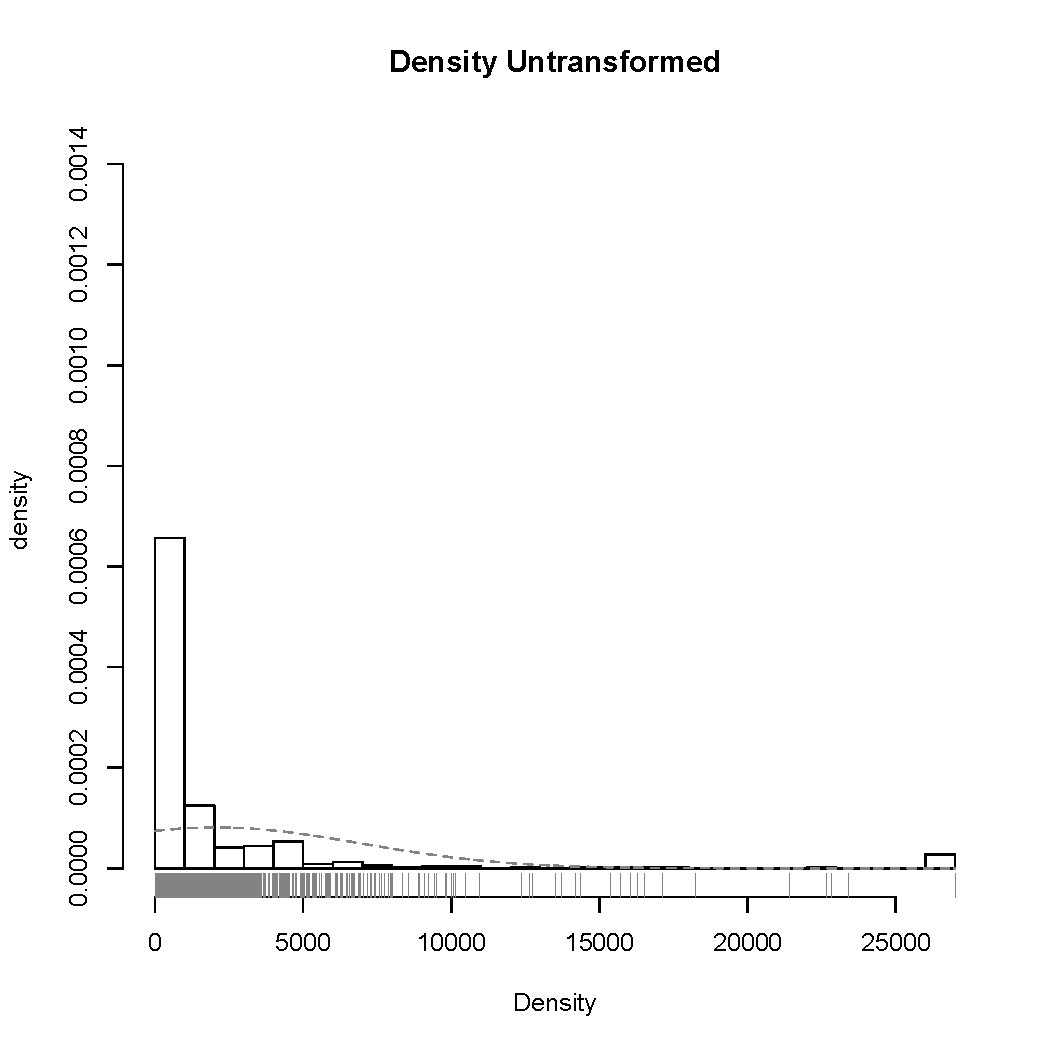
\includegraphics[scale=0.40]{Density.pdf}
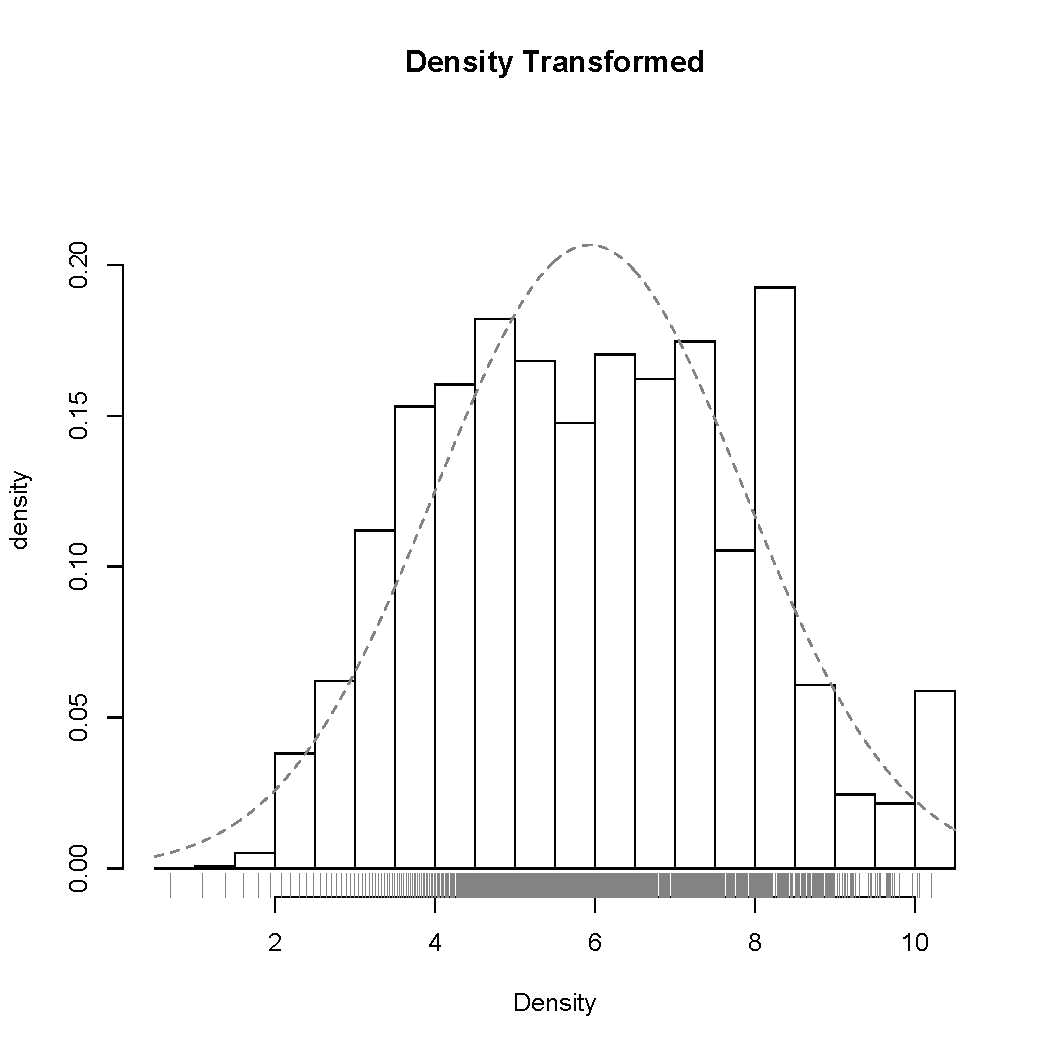
\includegraphics[scale=0.40]{logDensity.pdf}
\end{center}

\label{fig:vet1}
\end{figure}


Beginning with the continuous covariate $Density$, we want to inspect the shape of its univariate data to see if it follows Gaussian distribution. %Nik: use teletype for variable names , Paul: Like this? I am not sure what you mean by teletype, like telegraph type? or Mathematical type?
The left side of Figure \ref{fig:vet1} clearly revels that the the $Density$ is rather skewed right with several observations that report high value of density. This indicates a need for a transformation. With the log-normal assumption, the $Density$ is transformed which improves the fit (see the right side of Figure \ref{fig:vet1}) on the data.

\begin{table}[!htbp] \centering
  \caption{Comparing AIC and BIC for CWM verses GCWM models.}
  \label{comparingCWM_models}
\begin{tabular}{@{\extracolsep{5pt}} rrrr}
\\[-1.8ex]\hline
\hline \\[-1.8ex]
Model & k & AIC & BIC \\
\hline \\[-1.8ex]
CWM & $1$ & $$$352,470$ & $$$352,661$ \\
& $2$ & $$$314,560$ & $$$314,949$ \\
& $3$ & $$$301,223$ & $$$301,812$ \\
& $4$ & $$$287,020$ & $$$287,808$ \\
& $\bm{5}$ &$$$\bm{284,283}$ & $$$\bm{285,268}$ \\
GCWM & $1$ & $$$111,129$ & $$$111,320$ \\
& $2$ & $$$90,039$ & $$$90,428$ \\
& $3$ & $$$89,476$ & $$$90,065$ \\
& $\bm{4}$ & $$$\bm{88,781}$ & $$$\bm{89,568}$ \\
& $5$ & $$$88,731$ & $$ $89,717$ \\
\hline \\[-1.8ex]
\end{tabular}
\end{table}

The result of the transformation is a better AIC and BIC. Table \ref{comparingCWM_models} shows a considerable difference in BIC and AIC comparing CWM and GCWM. The five component CWM with a BIC of 285,268 is significantly higher than the four component GCWM with a considerably lower BIC of 89,568.

	We now investigate the results of GCWM in relation to the valuation of risk. For practical uses, finding clusters allows us to create different classifications of risk for various fields of drivers. The following GCWM allows to cluster different drivers in groups allowing one to assign different rates to different clusters.
\begin{figure}[!htb]
\caption{Showing clusters in color for Loss Amount vs Density on a log scale.}
\label{fig:vet1}
\begin{center}
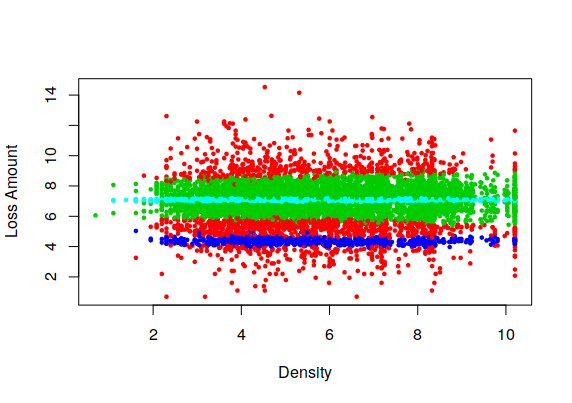
\includegraphics[scale=0.83]{SeverityPlot}
\end{center}
\end{figure}
\begin{table}[!htb]
\centering
\caption{Size of clusters for the GCWM a model.}
\label{table:sizeSev}
\begin{tabular}{rrrr}
\hline\hline
1   & 2  &  3   & 4    \\
1,683 & 5,766 & 848 & 7,093 \\
Red & Green & Blue & Teal \\
\hline\hline
\end{tabular}
\end{table}

After fitting the model, we then take a look at the size of each cluster. The GCWM approach has chosen four components as the best model to represent the data. The size of each cluster is displayed in Table \ref{table:sizeSev}. Attention is brought to largest quantity  of drivers that are grouped into cluster 4. This accounts for $ 46 \% $ of all drivers and is fairly concentrated in the center of Figure \ref{fig:vet1}.
From the results we can create an insurance model with the following characteristics. Cluster 3 drivers have both low variability and low average cost in claims, thus can be insured with a lower rate than other drivers. From a risk management perspective this is the most ideal case as these claims have very low variance and cost. Cluster 4 drivers have also low variability but a higher average cost, thus they would have a rate higher than cluster 3. Cluster 2 drivers have the next highest cost and variability of the clusters, these drivers are colored in green in Figure \ref{fig:vet1}. The final cluster colored in red has the highest cost and variaiblity in claims out of any of the other clusters. From a risk management perspective this cluster would have the highest rate.
\begin{table}[!htb]
\centering
\caption{Summarized volatility information of each cluster for Claims.}
\label{table:volSev}
\scalebox{0.90}{
\begin{tabular}{rrrrrr}
\hline\hline
Volatility Level - (Cluster)  $\quad$    & Minimum & Mean  & Maximum & $\sigma (0.05) $    \\
\hline
V1 - (3)$\quad\quad\quad$ & 51  & 79 & 154 & \textbf{ 13} \\
V2 - (4)$\quad\quad\quad$ & 1039  & 3109  &  1324 & \textbf{ 52} \\
V3 - (2)$\quad\quad\quad$ & 221 & 1687  & 8841  &\textbf{ 1284}  \\
V4 - (1)$\quad\quad\quad$ & 2 & 9717 & 2036833  & \textbf{ 64835}   \\
\hline\hline
\end{tabular}
}
\end{table}



Table \ref{table:volSev} shows a breakdown of the types of drivers, ordered by volatility in descending order. Beginning with V1, these drivers tend to have claims between \$51 to \$154, with a standard deviation of \$13, and a mean of \$79. That means that these drivers rarely exceed costs and tend to have very low volatility. Moving onto V2, these drivers have the second level of volatility. Drivers in this range tend to have claims anywhere between \$1039 to \$3109, with a standard deviation of \$ 52, and a mean of \$3109.  Proceeding to V3, its volatility in claims is greater than the preceding levels. Drivers in this cluster have claims anywhere between \$221 to \$8841, with a mean of \$1687, and a standard deviation of \$1284. Finally V4 denotes the level of highest volatility. Claims in this level  reach the highest recorded claim of \$ 2036833, a mean of \$9717, and a standard deviation of \$64835.

Coefficients of clustered results are used to calculate premiums in car insurance. Table \ref{severity_coef_table} shows the coefficients of the fitted model. The significance codes are defined as $  P < 0.001 : $  (***), $0.001 < P < 0.01:$ (**), $  0.01 < P < 0.05:$ (*), $0.05 < P < 0.10 : $ (.) %Nik: something wrong here; all of these could be considered $\approx 0$... use < some value.
pertaining to the $P$ value of the specific coefficient. In each cluster significance varies but overall the majority of coefficients are significant.

To summarize, the drivers have been clustered into four categories with distinct characteristics outlined in Table~\ref{table:volSev}. We have seen how using the results from GCWM, one can create an insurance model based on clustering algorithms with various levels of risk represented in each cluster. GCWM found a group that was the clear majority of drivers, in which the volatility of their claims was extremely low regardless of $Density$ or $DriverAge$ The results show that GCWM may potentially find unique clusters that are otherwise hidden within the data.


 \subsubsection{Modeling Claims Frequency}

In this section, we model frequency of the French motor claims. We consider the covariates density, driver age, car age, exposure and power. The choice of covariates stems from the previously modelled single component ZIP \citep{Charpentier:2014}.
The GCWM is modelled with the linear formula

\begin{equation}
Claim Nb = Density + Exposure + Power \quad|\quad Exposure + Car Age
\end{equation}

where $Density$, $Exposure$, and $Power$ models  Poisson, while $Exposure$ and $Car Age$ models Bernoulli. As in Section 4.2.1, we also impose a log-normal assumption on the $Density$ covariate.
After fitting the model, GCWM has found two zero-inflated components and one Poisson component as the best model to represent the data. The size of each cluster is displayed in Table~\ref{table:sizeFreq}. We note a fairly even spread of the size across the three clusters.

 \begin{table}[!htb]
\centering
\caption{Size of clusters for the GCWM a model.}
\label{table:sizeFreq}
\begin{tabular}{rrrr}
\hline\hline
1   & 2  &  3   \\
100492 & 163503 & 149174 \\
Red & Green & Blue  \\
\hline\hline
\end{tabular}
\end{table}

\begin{figure}[!ht]
\begin{center}
\caption{Showing clusters in color for Frequency vs Density under lognormal assumptions.}
\label{frequencyGraph}
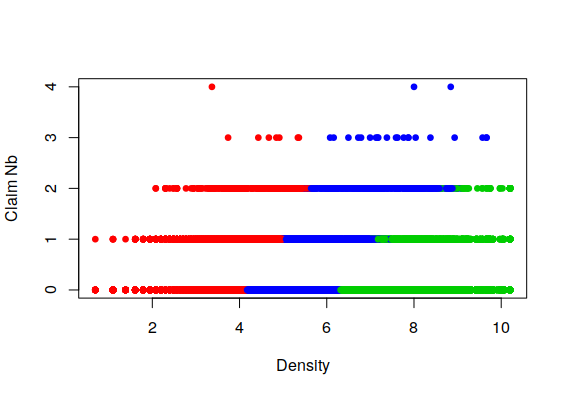
\includegraphics[scale=0.80]{frequency.png}
\end{center}
\end{figure}
% Nik To Paul: Should I put a title on the plot just like the severity one before? or should I remove the title of the severity figure

Similarly to modelling severity, the GCWM finds clusters with unique characateristics. This is evident when looking at the Claims vs. Density plot in Figure \ref{frequencyGraph}. We see that the GCWM has split up the drivers into three groups based on the Density of cities. Table \ref{summarycovariates} shows that cluster 2 drivers live in the least dense cities with a mean of 7.86 km on the log scale. Followed by clusters 3 and 1 with a mean of 5.23 km and 3.38 km respectively.

 \begin{table}[!htb]
 \begin{center}
 \caption{Summary of each cluster with log-normal assumptions for the Density covariate (log scale).} \label{summarycovariates}
\begin{tabular}{rrrrr}
\hline
\hline
Cluster - Color & Minimum (km) & Mean (km) & Maximum (km) & $\sigma$ (km) \\
\hline
1 - Red         & 0.69    & 3.38 & 5.60    & 0.60  \\
2 - Green       & 6.29    & 7.86 & 10.20   & 1.03  \\
3 - Blue        & 4.13    & 5.23 & 9.66    & 0.65 \\
\hline\hline
\end{tabular}
\end{center}
\end{table}

Table \ref{frequencySummary} shows a summary of the coefficients for the zero-inflated model. The
significance codes are the same as of Table \ref{severity_coef_table}. In each cluster we can see that the majority of the coefficients are signficant particularly in the zero-count model for Bernoulli. Cluster 1 was selected to be strictly a Poisson model by the liklihood ratio test defined in \eqref{LRTest}. In summary we see that the GCWM can account for zero-inflated data in pricing.


\section{Simulation Study}

Two simulation studies are conducted to determine the validity of the log-normal assumption and the effectiveness of the Bernoulli-Poisson partitioning method. The first section outlines the need for a non-gaussian assumption for the covariates. The second section shows the classification accuracy and other relevant analysis for the Bernoulli-Poisson method.


\subsection{Simulation Study - GCWM}


In this section, we show how the proposed methodology works for different simulation settings. The simulation study was generated based on the regression coefficients of the \textbf{CASdataset} used in the previous section. The aim of the simulation study was to test the accuracy and ability of both GCWM a and CWM to return estimates of true parameters when one or more of the covariates is lognormal and the other two are Gaussian. This was designed to test both functions in the event when one of the covariates is non-Gaussian. The motivation behind this is fact is that many covariates used in insurance are likely to come from non-Gaussian distribution. Thus this was aimed to test the relevancy of CWM, which treats all covariates as Gaussian.

We define Model 1 as the base line model in which the coefficients were generated for \textbf{CASdataset} and reported in upper portion of Table 2. These coefficients were then rounded and treated as true parameters. A simulation with three GLM mixture components was then generated around these true parameters in which the third covariate $X_3$ was lognormal. Stemming from this, both CWM and  GCWM a were run. The  GCWM a treats $X_3$ as a lognormal covariate. 

The results for Model 1 were summarized in upper portion of Table 3 based on the performance of the  GCWM a approach. The simulation was run $1000$ times. We reported the percentage of runs for each predictor and the corresponding intercept in each mixture component under the assumption of $5\%$ error. For example, predictor $X_2$ in the component 2 of Model 1 reported $90.10\%$ accuracy. This means that $90.1\%$ of the time the true parameter was estimated within $5\%$ error. In this setting, predictor $X_1$ in the second component was insignificant in the real data set. The purpose of including this parameter in Model 1 was to test the sensitivity of  GCWM a for insignificant predictors. In this case, the result of zero is underlined and it means that it has no influence on the response variable in this simulation. Further, we created Models 2, 3, 4 and 5 by altering the parameters of Model 1 by $+30\%$, $-30\%$, $+50\%$, and $-50\%$ accordingly and keeping the second covariate of the second component as an insignificant predictor form the \textbf{CASdataset} model. This was done to test the accuracy of  GCWM a to the  sensitivity of coefficients. Based on the results in Table 3, we can see that  GCWM a performs well for all simulation settings.




\begin{center}
\begin{table}[!htb]
\label{my-label}
\caption{GCWM a vs CWM Accuracy: Covariate $X_3$ is treated as log-normal, the rest are Gaussian covariates.}
\begin{adjustwidth}{-1cm}{}
\begin{tabular}{|rrrrrr|rrrr|}
\hline\hline
Model & Component & Intercept & $X_1$ &$X_2$ & $X_3$& Intercept & $X_1$ &$X_2$ & $X_3$  \\
\hline
1     & 1         & 93.00\%   & 90.10\%  & 93.00\%  & 93.10\% & 0.00\% & 0.00\% & 0.00\% & 0.00\%   \\
      & 2         & 90.10\%   & \underline{0.00\%}   & 90.10\%  & 90.10\% & 0.00\% & 0.00\% & 0.00\% & 0.00\%  \\
      & 3         & 99.20\%   & 99.10\%  & 99.20\%  & 99.20\% & 0.00\% & 0.00\% & 0.00\% & 0.00\%  \\
2     & 1         & 89.80\%   & 89.20\%  & 89.80\%  & 89.80\% & 0.00\% & 0.00\% & 4.60\% & 0.00\%  \\
      & 2         & 89.20\%   &\underline{0.00\%}   & 89.20\%  & 89.20\% & 0.00\% & \underline{0.00\%} & 0.00\% & 0.00\%   \\
      & 3         & 99.20\%   & 99.20\%  & 99.20\%  & 99.20\% & 0.00\% & 0.20\% & 1.70\% & 0.00\%  \\
3     & 1         & 100.00\%  & 100.00\% & 100.00\% & 100.00\%  & 0.00\% & 0.00\% & 0.00\% & 0.00\% \\
      & 2         & 100.00\%  & \underline{0.00\%}   & 100.00\% & 100.00\% & 0.00\% & 0.00\% & 0.00\% & 0.00\% \\
      & 3         & 99.20\%   & 99.20\%  & 99.20\%  & 99.20\%  & 0.00\% & 0.00\% & 0.00\% & 0.00\%\\
      4 & 1 & 88.60\% & 86.80\% & 88.60\% & 87.00\%  & 0.00\% & 0.00\% & 0.00\%  & 0.00\%  \\
  & 2 & 86.90\% &\underline{ 0.00\%}  & 86.90\% & 86.90\% & 0.00\% & \underline{0.00\%} & 0.00\%  & 0.00\%  \\
  & 3 & 99.20\% & 99.20\% & 99.20\% & 99.20\% & 0.00\% & 0.00\% & 0.00\%  & 0.00\% \\
5 & 1 & 85.90\% & 84.90\% & 85.60\% & 85.90\% & 0.00\% & 0.00\% & 0.00\%  & 0.00\% \\
  & 2 & 85.00\% &\underline{ 0.00\%}  & 84.90\% & 84.90\% & 0.00\% & \underline{0.00\%} & 0.00\%  & 0.00\%  \\
  & 3 & 99.20\% & 99.20\% & 99.20\% & 99.20\% & 0.00\% & 0.20\% & 10.90\% & 0.00\% \\
      \hline\hline
\end{tabular}
\end{adjustwidth}
\end{table}
\end{center}


Table 4 provides the summary of the results when CWM was used in the analysis of the same models considered in Table 3. It is not surprising to see that barely any of the simulation runs estimated correctly all parameters as most of the results are zero. This means that the performance of CWM approach is poor in presence of one non-Gaussian covariate which in this case is a log-normal covariate. Similarly to Table 3, Table-4 shows the underlined results pointing to insignificant predictors.

\begin{table}[!htb]
\centering
\caption{ GCWM a results: the summary of MSE for all parameters used in five models. The covariate $X_3$ is treated as log-normal a nd the rest are Gaussian. These results correspond to those in Table 3.}
\label{my-label}
\begin{tabular}{rrrrrrrrrr}
\hline\hline
Model & Component & $\beta_o$ &  MSE($\beta_o$)   &  $\beta_1$ & MSE($\beta_1$)& $\beta_2$ &MSE($\beta_2$)   & $\beta_3$ &  MSE($\beta_3$)  \\
\hline
1     & 1         & 1028& (11.353)   & 0.03& (0.00)  & 3.5& (0.00)    & -380& (0.09)   \\
      & 2         & 1600& (0.000)     & -0.01&(0.00) & 1.5&(0.00)    & -250&(0.00)   \\
      & 3         & 40000&(0.035)    & -6.00&(0.00) & -305&(0.00) & 1100&(0.47)   \\
2     & 1         & 1350&(0.167)     & 0.04&(0.00)  & 4.5&(0.00)    & -500&(0.03)   \\
      & 2         & 2080& (0.001)     & 0.04&(0.00)  & 2.0&(0.00)    & -325&(0.00)   \\
      & 3         & 52000& (0.012)    & -8.00&(0.00) & 450&(0.00)  & 14300&(0.01)  \\
3     & 1         & 720& (0.001)      & 0.02&(0.00)  & 2.5&(0.00)   & -266&(0.00)   \\
      & 2         & 1100& (0.008)     & 0.00&(0.00)  & 1.1&(0.00)    & -17511&(0.00) \\
      & 3         & 28000& (0.002)    & -4.20&(0.00) & 245&(0.00)  & 7700.&(0.00) \\
4     & 1         & 1650&(13.056)   & 0.05&(0.00)  & 5.3&(0.00)    & -570&(0.00)   \\
      & 2         & 2400& (0.000)     & -0.01&(0.00) & 2.3&(0.00)    & -375&(0.00)   \\
      & 3         & 60000& (0.051)    & -9.00&(0.00) & -457&(0.00) & 16500&(0.00)  \\
5     & 1         & 500& (1.115)     & 0.02&(0.00)  & 2.0&(0.00)    & -190&(0.05)   \\
      & 2         & 800& (0.003)      & 0.00&(0.00)  & 0.8&(0.00)    & -120&(0.00)   \\
      & 3         & 20000& (0.000)    & -3.00&(0.00) & -150&(0.00) & 5500&(0.00)  \\
      \hline\hline
\end{tabular}

\end{table}







Table 5 provides the summary of Mean Squared Errors (MSE) of each parameter of the models in Table 3 estimated via 1000 simulation runs. The MSE is computed using the following formula MSE$(\beta_i) = \frac{\sum_i^n (\beta_i - \hat\beta_i ) ^2}{n}$. The MSEs related to the predictor variables for all models and their corresponding components are about zero indicating that  GCWM a approach performs well. This is also a result of having a small size coefficients.


\begin{table}[!htb]
\centering
\caption{CWM results: the summary of MSE for all parameters used in five models. All three covariates are treated as Gaussian. These results correspond to those in Table 4.}
\label{my-label}
\begin{tabular}{rrrrrrrrrrrr}
\hline\hline
Model & Component & $\beta_o$ &  MSE($\beta_o$)   &  $\beta_1$ & MSE($\beta_1$)& $\beta_2$ &MSE($\beta_2$)   & $\beta_3$ &  MSE($\beta_3$)  \\
\hline
1     & 1         & 1028& ($\cdot$)   & 0.03&  ($\cdot$)   & 3.5&  ($\cdot$)    & -380&  ($\cdot$)    \\
      & 2         & 1600&  ($\cdot$)      & -0.01& ($\cdot$)  & 1.5& ($\cdot$)     & -250& ($\cdot$)  \\
      & 3         & 40000& ($\cdot$)     & -6.00& ($\cdot$)  & -305& ($\cdot$)  & 1100& ($\cdot$)    \\
2     & 1         & 1350& ($\cdot$)     & 0.04& ($\cdot$) & 4.5& ($\cdot$)    & -500& ($\cdot$)  \\
      & 2         & 2080&  ($\cdot$)    & 0.04& ($\cdot$)   & 2.0& ($\cdot$)     & -325& ($\cdot$)   \\
      & 3         & 52000&  ($\cdot$)     & -8.00& (0.006)  & 450& (44.1)   & 14300& ($\cdot$)  \\
3     & 1         & 720&  ($\cdot$)     & 0.02& ($\cdot$)   & 2.5& ($\cdot$)    & -266& ($\cdot$)    \\
      & 2         & 1100&  (65.814)     & 0.00& ($\cdot$)   & 1.1& ($\cdot$)     & -17511& ($\cdot$)  \\
      & 3         & 28000& ($\cdot$)   & -4.20& ($\cdot$)  & 245& ($\cdot$)   & 7700.& ($\cdot$)  \\
4     & 1         & 1650& ($\cdot$)    & 0.05& ($\cdot$)  & 5.3& ($\cdot$)    & -570& ($\cdot$)  \\
      & 2         & 2400&  ($\cdot$)     & -0.01& ($\cdot$)  & 2.3& ($\cdot$)    & -375& ($\cdot$)    \\
      & 3         & 60000&  ($\cdot$)     & -9.00& ($\cdot$)  & -457& ($\cdot$)  & 16500& ($\cdot$)   \\
5     & 1         & 500&  ($\cdot$)     & 0.02& ($\cdot$)   & 2.0& ($\cdot$)   & -190& ($\cdot$)  \\
      & 2         & 800&  ($\cdot$)      & 0.00& ($\cdot$)   & 0.8& ($\cdot$)    & -120& ($\cdot$)  \\
      & 3         & 20000&  ($\cdot$)     & -3.00& (0.003)  & -150& (4.7) & 5500& ($\cdot$) \\
      \hline\hline
\end{tabular}
\end{table}








Table 6 provides the summary of Mean Squared Errors (MSE) of each parameter of the models in Table 4 estimated via 1000 simulation runs.
In contrary to the results reported in Table 5, these results in Table 6 are significantly different. We can observe that the MSEs for most of the Models and their corresponding coefficients are not calculated at all due to convergence failures and as such they are shown as $(\cdot)$. This is not surprising because Table 4 shows the accuracy of CWM is not good when attempting to model non-Gaussian predictors as Gaussian.

In summary, our simulation results showed good performance of the GCWM approach in modeling non-Gaussian covariates. More specifically, these results show high accuracy when covariates are log-normal. In contrary, CWM fails to estimate parameters accurately when the Gaussian assumption is violated.

\subsection{Simulation Study - Bernoulli-Poisson Partitioning}

In this section we show how the Bernoulli-Poisson partitioning (BP) method  behaves under different conditions. The components were genereated under similar coefficients taken from the \textbf{CASDatasets} package. The coefficients were rounded and treated as true parameters to which data was generated from. The mean and standard deviation of the covariates within each component was also taken into account when generating data. The first simulation examines the performance of the GCWM a model for classification. We generate three components each with sample size $N=1000$ for a total of $3000$ simulated points.
The model generated is similar to the mean and standard deviations of Table \ref{summarycovariates}. Consider three simulated covariates and 
\begin{equation}
SimClaimsNb = SimDriverAge + SimDensity + SimCarAge 
\end{equation}
as the GLM. The covariates $SimDriverAge$,$SimDensity$,and $SimCarAge$ are considered for both the Poisson and Bernoulli models. 
 Here the GCWM is fitted to the simulated data and used to classify into three components. The misclassification rate is calculated by the proportion of true labels placed in other components by the GCWM a model.  The results of the simulation is based on the generated dataset are presented in Table \ref{misclassTable}. The total misclassification rate  is $1.8 \% $ and the majority of misclassified components are between components two and three.
\begin{table}[!htb]
\begin{center}
\caption{Misclassfication rate and label comparison of generated data.}
\label{misclassTable}
\begin{tabular}{r r r r r r}
\hline\hline
    True Labels       &  \multicolumn{3}{r}{ Classified }   & Misclassification Rate  &  \\ \cmidrule{2-4}
   & 1                              & 2   & 3   &                            &  \\ \hline
1              & 992                            & 3   & 5   & 0.80 \%                                      &  \\
2              & 0                              & 990 & 10  & 1.00 \%                                       &  \\
3              & 15                             & 20  & 965 & 3.50 \%                                      &  \\  \hline
                \multicolumn{4}{r}{Overall Misclassification Rate}        & 1.80 \%                  & \\
        		\multicolumn{4}{r}{Average Purity} & 98.23 \%  
        		\\ \hline
                \multicolumn{4}{r}{Adjusted Rand Index} & 0.9479 &  \\
    \hline\hline
\end{tabular}
\end{center}
\begin{align*}
n_{ij} &= \text{ across diagonal }, \quad\quad  a_i = \text{ row sums }, \quad\quad b_j = \text { column sums } \\
 ARI &= \frac{ \sum_{ij} \binom{n_{ij}}{2} - [\sum_i \binom{a_i}{2} \sum_j \binom{b_j}{2}] / \binom{n}{2} }{ \frac{1}{2} [\sum_i \binom{a_i}{2} + \sum_j \binom{b_j}{2}] - [\sum_i \binom{a_i}{2} \sum_j \binom{b_j}{2}] / \binom{n}{2} } \quad\quad AP = \frac{1}{N} \sum_i  n_{ij}
\end{align*}
\end{table}

The experiment is expanded further to show how Bernoulli-Poisson partitioning behaves over 1000 runs and under two different conditions. The first condition is defined as follows. The mean and standard deviations are taken as given by the estimated  ZIP components from the \textbf{CASDataset}. The second condition involves adjusting the means of two of the covariates so they are closer to each other. The goal is to show that the BP-method holds its use even when means among covariates are close.  Conditions are divided into two categories. N is considered normal, where the covariate means are taken directly from the sample data. C is considered to be ``close", where the covariate means are manipulated so that they are closer to each other within some degree. This is a common problem in classification where if the means among two different components are close, then misclassification rate increases [\cite{LimHwa}]. Experiment 2 defines the use of 3 different partitioning methods to initialize a zero-inflated model. Poisson method assumes that the presence of non-zeros will provide a better partitioning of the data-set. Bernoulli assumes that the presence of excess zeros will determine the best partitioning of the data-set . Finally the BP-Method assumes that both methods are weighed equally and therefore both must be taken into account when partitioning the dataset. The mean and standard deviation of each measurement is provided in Table \ref{table:exper2}.

\begin{table}[!htb]
\begin{center}
\caption{Experiment 2: mean and standard deviations for each statistic comparing each method.}
\label{table:exper2}
\begin{tabular}{rrrrrrrr}
\hline\hline
Type   & Condition & Poisson & ($\sigma $) & Bernoulli & ($ \sigma $) & BP-Method & ($ \sigma $) \\
\hline
Misclassification Rate& N         & 1.70\% & (6.00)       & 1.60\%  & (6.00)         & 1.10\% & (0.02)         \\
       & C         & 5.00\% & (7.00)       & 6.00\% & (2.00)         & 7.00\% & (4.00)         \\
Average Purity & N         & 98.87\% & (2.00)    & 98.91\% & (2.25)      & 99.18\% & (0.81)     \\
       & C         & 95.38\% & (4.00)    & 94.55\% & (1.00)      & 96.95\% & (0.48)      \\
Adjusted Rand Index  & N         & 0.9662 & (0.07)    & 0.9677  & ( 0.07)     & 0.9729 & (0.0217)      \\
       & C         & 0.8706 & (0.08)    & 0.8366 & (0.04)      & 0.8538 & ( 0.0453) \\
       \hline\hline
\end{tabular}
\end{center}
\end{table}
Several findings are concluded from Table \ref{table:exper2}. Under condition N, the BP method shows better performance in error and is found to be less sensitive than other methods with an error rate of $ 1.10 \% $ and a standard deviation of $ 0.02 \% $.  Further findings show that when condition C is imposed then Bernoulli has better performance in terms of accuracy. The ARI shows good measurements overall however the BP-Method under condition N has a very good ARI with a small standard deviation. The Average Purity of the BP-Method is the best out of all other methods, which is relevant to estimating coefficients accurately for optimization.

\section{Conclusion}

In this paper, we extend the class of generalized linear mixture CWM models by accomplishing two main goals. First, we proposed the methodology that allows for continuous covariates to follow a non-Gaussian distribution. Imposing Gaussian distribution on a skewed data may result in an suboptimal model fit. Second, we proposed a new Poisson CWM methodology that uses Bernoulli-Poisson partitioning and allows for implementation of zero-inflated Poisson CWM model (ZI-GCWM). We call our proposed model class GCWM, which reflects two extensions made to the existing CWM class of models.

Our proposed GCWM models allow for great applications in predictive modeling of insurance claims by overcoming a few limitations of the current CWM models. The ZI-GCWM allows for finding clusters within claims frequency which is an important information in risk classification and modeling of claims frequency. Further, some insurance rating variables used in the predictive modeling of severity claims may not strictly follow Gaussian assumptions, e.g. driver's age or car age (treated as continuous covariates). An adequate extension to non-gaussian covariates can be considered to relax current assumptions and improve the model fit. We demonstrated that there is a need for a log-normal assumption which can be considered easily to improve the model fit.

The results of our extensive simulation study showed the excellent performance of the proposed models in case of modeling non-Gaussian covariates. We found  that current CWM model fails to estimate the parameters accurately when the Gaussian assumption is violated. The GCWM a shows significant improvement in the model fit over the CWM model based on AIC and BIC criteria. We also tested Bernoulli-Poisson partitioning of zero-inflated GCWM under different conditions and found that our proposed partitioning method has a very low misclassification rate, high average purity, and high average rand index.

Our approach is relevant to the actuarial pricing and risk management when current practices are based on implementation of various GLM models. Further extension of this work may incorporate modifications of the CWM family to allow for modeling limited depended variable or the right-censored data structure (refer to \cite{miljkovic2015} and \cite{miljkovic+orr:2017}).



\newpage
\section{Appendix}

\subsection{Derivation of the Log-normal Distribution }
Consider a random variable $U$ having univariate log-normal distribution with parameters $\mu \in \mathbb{R}$ and $\sigma \in \mathbb{R}_+ $. Have $u \in \mathbb{R}_+$, then the probability density function of random variable $U$ is defined as \footnote{For full definition see \cite{johnson1995continuous}}
$$\mathcal{LN}(u; \mu, \sigma) = \frac{1}{u\sigma\sqrt{2\pi}}\exp\left[-\frac{(\ln u - \mu)^2}{2\sigma^2}	\right].$$
\text{Further, if random variable }$X$\text{ is normally distributed i.e. }$ X \sim \mathcal{N}(x; \mu, \sigma) $, then $U := \exp{(X)}\sim \mathcal{LN}(u; \mu, \sigma) $.
To see this, let $p_U(u)$, and $ p_X(x) $ be the probability density functions of $U$ and $X$ respectively. By the change of variables theorem (see \cite{murphy2012machine} section 2.6.2.1) the density $p_U(u)$ is derived as
$$p_U(u) = p_X(\ln u )\frac{\partial}{\partial u} \ln u  =  p_X(\ln u ) \frac{1}{u} =  \frac{1}{u\sigma\sqrt{2\pi}}\exp\left[-\frac{(\ln u - \mu)^2}{2\sigma^2}	\right].$$\newline
 We extend to a log-normal multivariate case where the random variable $\bm{U} $ is parameterized by $ \bm{\mu} \in \mathbb{R}^p$ and $\bm{\Sigma} \in  \mathbb{R_{+}}^p \label{changeVarUni} $.
\begin{lemma}
Let the random variable $\bm{X}$ have multivariate normal distribution ie. $\bm{X} \sim \mathcal{MVN}(\bm{x}, \bm{\mu},\bm{\Sigma}) $, then $\bm{U} := \exp(\bm{X} ) \sim  f^U(\bm{u}; \bm{\mu } , \bm{\Sigma} )$. Here
have $\bm{u} \in \mathbb{R_{+}}^p $ and the probability density function $f^U$ is
$$ f^U(\bm{u}; \bm{\mu } , \bm{\Sigma} )= \frac{1}{(\prod_{i=1}^{N}u_{i})| \bm{\Sigma} |(2 \pi)^{\frac{p}{2}}}   \exp\left[-\frac{1}{2}(\ln \bm{u} -\bm{\mu})^{'}  \bm{\Sigma^{-1}}(\ln \bm{u} -\bm{\mu})\right].  $$
\end{lemma}
\begin{proof}
Let $f^U(\bm{u}; \bm{\mu},\bm{\Sigma})$ and $f^X(\bm{x}; \bm{\mu},\bm{\Sigma})$ be the probability density functions of $\bm{U}$ and $\bm{X}$ respectively. By the multivariate change of variables theorem (see \cite{murphy2012machine} section 2.6.2.1), we derive the log-normal distribution, where $ | \det J_{\ln} (u) | $ is the absolute value of the determinant for the Jacobian of the multivariate transformation $\ln(\bm{U}) = \bm{X} $. Hence,
\begin{align*}
 | \det J_{\ln} (\bm{u}) | & = \prod_{i=1}^n u_i^{-1}, \; \text{and} \; \\
   f^U(\bm{u}; \bm{\mu},\bm{\Sigma})  & =  f^X(\ln \bm{u}; \bm{\mu},\bm{\Sigma})  | \det J_{\ln} (u) | \\
  & = f^X(\ln \bm{u}; \bm{\mu},\bm{\Sigma})\prod_{i=1}^n u_i^{-1} \\
  & =  \frac{1}{(\prod_{i=1}^{N}u_{i})| \bm{\Sigma} |(2 \pi)^{\frac{p}{2}}}   \exp\left[-\frac{1}{2}(\ln \bm{u} -\bm{\mu})^{'}  \bm{\Sigma^{-1}}(\ln \bm{u} -\bm{\mu})\right].
  \end{align*}
\end{proof}


\begin{center}
\begin{sidewaystable}
\caption{Summary of coefficients for severity clusters.}
\label{severity_coef_table}
\begin{tabular}{|l|rrc|rrc|rrc|rrc|}
\hline\hline
         & V1         & (Red)     &    & V2         & (Green)   &    & V3          & (Blue)     &    & V4          & (Teal)     &    \\
Coef      & Estimate   & Error     & P   & Estimate   & Error     & P   & Estimate    & Error      & P   & Estimate    & Error      & P   \\ \hline
Intercept & 7.876  & 0.137 & *** & 7.180  & 0.061 & *** & 4.673   & 0.014 & *** & 7.077  & 0.003 & *** \\
Density   & -0.031 & 0.009 & *** & 0.005  & 0.004 &     & -0.011 & 0.001 & *** & 0.002  & 0.002 &     \\
C2        & -0.172 & 0.080 & *   & 0.064  & 0.034 & .   & 0.020 & 0.001 & **  & 0.008  & 0.002 & *** \\
C3        & -0.396 & 0.080 & *** & 0.108  & 0.034 & **  & 0.010  & 0.007 &     & 0.003  & 0.002 & .   \\
C4        & -0.642 & 0.081 & *** & -0.033 & 0.035 &     & 0.034  & 0.007 & *** & 0.005  & 0.002 & **  \\
C5        & -0.500 & 0.090 & *** & 0.066 & 0.039 & .   & 0.069  & 0.007 & *** & 0.011  & 0.002 & *** \\
D2        & -0.535 & 0.083 & *** & -0.168 & 0.038 & *** & -0.217 & 0.009 & *** & -0.006 & 0.001 & *** \\
D3        & -0.607  & 0.084 & *** & -0.241 & 0.038 & *** & -0.205 & 0.009 & *** & -0.008 & 0.001 & *** \\
D4        & -0.390 & 0.099 & *** & -0.122 & 0.045 & **  & -0.200 & 0.0106 & *** & -0.009  & 0.002 & *** \\
D5        & 0.123 & 0.101 &     & 0.035  & 0.047 &     & -0.138 & 0.010 & *** & -0.002 & 0.002 &     \\
R23       & 0.003 & 0.131  &     & -0.016 & 0.053 &     & -0.001 & 0.012 &     & 0.002  & 0.006 &     \\
R24       & -0.232 & 0.054 & *** & -0.017 & 0.023 &     & -0.102 & 0.005 & *** & -0.015 & 0.013 & *** \\
R25       & 0.144  & 0.096 &     & -0.184 & 0.043 & *** & -0.065 & 0.009 & *** & -0.016 & 0.024 & *** \\
R31       & -0.009 & 0.073 &     & 0.055  & 0.031 & .   & -0.141 & 0.008 & *** & -0.003 & 0.018 & .   \\
R52       & -0.303 & 0.064 & *** & 0.012   & 0.028 &     & -0.142 & 0.006  & *** & -0.015 & 0.038 & *** \\
F53       & -0.153 & 0.063 & *   & 0.095  & 0.028 & *** & -0.012 & 0.006  & *   & -0.014 & 0.001 & *** \\
R54       & -0.222 & 0.082 & **  & 0.074  & 0.037 & *   & -0.122 & 0.007 & *** & -0.015  & 0.002 & *** \\
R72       & -0.098 & 0.072 &     & 0.175  & 0.031 & *** & -0.081 & 0.007 & *** & -0.007 & 0.002 & *** \\
R74       & -0.236 & 0.142 & .   & -0.114 & 0.067 & .   & 0.466  & 0.016 & *** & -0.019 & 0.003 & *** \\
P-FGH     & 0.123 & 0.033 & *** & 0.012 & 0.015 &     & 0.001    & 0.003 &     & 0.002  & 0.001 & *   \\
P-Other   & 0.131  & 0.045 & **  & 0.075   & 0.020 & *** & 0.012  & 0.003 & **  & 0.005  & 0.001  & *** \\
GR        & -0.095 & 0.031 & **  & -0.029 & 0.014 & *   & 0.005   & 0.002 & .   & -0.005 & 0.001 & *** \\
\hline\hline
\end{tabular}
\end{sidewaystable}

\begin{sidewaystable}
\caption{Summary of coefficients for frequency clusters.}
\label{frequencySummary}
\begin{tabular}{|l|rrc|rrc|rrc|}
\hline\hline
          & Cluster 1 & (Red) &   & Cluster 2 & (Green) &  & Cluster 3 & (Blue) &   \\
Coef        & Estimate  & Error & P   & Estimate  & Error   & P   & Estimate  & Error  & P  \\
 \hline
(Intercept) & -10.199   & 0.109 & *** & -7.217    & 0.216   & *** & -13.694   & 0.099  & *** \\
Density     & 1.860     & 0.027 & *** & 0.442     & 0.013   & *** & 1.771     & 0.013  & *** \\
Exposure    & 0.825     & 0.040 & *** & 0.726     & 0.192   & *** & 0.745     & 0.046  & *** \\
P-GH        & -0.063    & 0.030 & *   & -0.004    & 0.035   &     & 0.013     & 0.030  &     \\
P-Other     & -0.019    & 0.042 &     & 0.049     & 0.043   &     & 0.107     & 0.040  & **  \\
\hline
(Intercept) &          &      &    & 2.424     & 0.188   & *** & 1.886     & 0.356  & *** \\
Exposure    &          &      &    & -5.871    & 0.758   & *** & 16.520    & 2.990  & *** \\
C2          &          &      &    & -0.541    & 0.176   & **  & -0.922    & 0.368  & *   \\
C3          &          &      &    & -1.217    & 0.201   & *** & -2.263    & 0.553  & *** \\
C4          &          &      &    & -1.265    & 0.225   & *** & 10.805    & 72.677 &     \\
C5          &          &      &    & -0.808    & 0.266   & **  & -6.355    & 30.867 &   \\
\hline\hline
\end{tabular}
\end{sidewaystable}
\end{center}

\bibliographystyle{elsart-harv}
\bibliography{GLM_Mixtures_2018}

\end{document}


